\documentclass[12pt,a4paper,openany]{article}
%%%% JNLP 
\usepackage{lmodern}
\usepackage{xcolor}
\usepackage[utf8]{inputenc}
\usepackage[T1]{fontenc}
\usepackage[francais]{babel}
\usepackage[top=1.7cm, bottom=1.7cm, left=1.5cm, right=1.5cm]{geometry}
\usepackage{pdfpages}
\usepackage{listingsutf8}
\usepackage{fancyhdr}
\usepackage{multido}
\usepackage{amssymb}
\usepackage{tikz}
\usepackage{makeidx}
\usepackage[urlbordercolor={1 1 1}]{hyperref}


\date{\today}

\chead{Ce document est un outil pédagogique, il ne vaut en aucun cas contrat}
\rhead{}
\lhead{}
\makeindex
\lfoot{Université Paul Sabatier Toulouse III}
\rfoot{--~\thepage~--}
\cfoot{}
\makeglossary
\makeatletter
\def\clap#1{\hbox to 0pt{\hss #1\hss}}%
\def\ligne#1{%
\hbox to \hsize{%
\vbox{\centering #1}}}%
\def\haut#1#2#3{%
\hbox to \hsize{%
\rlap{\vtop{\raggedright #1}}%
\hss
\clap{\vtop{\centering #2}}%
\hss
\llap{\vtop{\raggedleft #3}}}}%
\def\bas#1#2#3{%
\hbox to \hsize{%
\rlap{\vbox{\raggedright #1}}%
\hss \clap{\vbox{\centering #2}}%
\hss
\llap{\vbox{\raggedleft #3}}}}%
\def\maketitle{%
\thispagestyle{empty}\vbox to \vsize{%
\haut{}{\@blurb}{}
\begin{flushleft}
	\vspace{1cm}
	Antoine de \bsc{Roquemaurel}\\ 
	Mathieu \bsc{Soum}\\
	Geoffroy \bsc{Subias}\\
	Marie-Ly \bsc{Tang}\\
	\textit{Groupe B}\\
\end{flushleft}
\begin{flushright}
	\vspace{-3cm}
	Pour Monsieur \bsc{Millan} (Client)\\
	Pour Madame \bsc{Kross} (Tuteur) \\
	Pour Monsieur \bsc{Marquié} (Correcteur)

\end{flushright}
\vfill
\vspace{1cm}
\begin{flushleft}
\usefont{OT1}{ptm}{m}{n}
\huge \@title
\end{flushleft}
\par
\hrule height 4pt
\par
\begin{flushright}
\usefont{OT1}{phv}{m}{n}
\Large \@author
\par
\end{flushright}
\vspace{1cm}
\vfill
\vfill
\bas{}{\@location, le \@date}{}
}%
\cleardoublepage
}
\def\date#1{\def\@date{#1}}
\def\author#1{\def\@author{#1}}
\def\title#1{\def\@title{#1}}
\def\location#1{\def\@location{#1}}
\def\blurb#1{\def\@blurb{#1}}
\date{\today}
\author{}
\title{}
\location{Amiens}\blurb{}
\makeatother
\title{Cahier des Charges Fonctionnel}
\author{Bibliothèque d'objets graphiques UML}

\location{Toulouse}
\blurb{%
Université Paul Sabatier -- Toulouse III\\
IUT A - Toulouse Rangueil\\
\textbf{Projet tutoré}\\[1em]
}%



\pagestyle{fancy}
\begin{document}
	\maketitle
	\newpage
	\tableofcontents
	\newpage
	\section{Contexte}
	\subsection{Présentation du groupe projet}
	Notre groupe projet est composé de quatre étudiants de deuxième année de DUT\footnote{Diplôme Universitaire de Technologie} Informatique à l'IUT\footnote{Institut Universitaire de Technologie} A de Toulouse, voici la composition de l'équipe: 
	\begin{itemize}
		\item Antoine de \bsc{Roquemaurel} 
		\item Mathieu \bsc{Soum} 
		\item Geoffroy \bsc{Subias}
		\item Marie-Ly \bsc{Tang} 
	\end{itemize}
	Nous avons monté ce groupe, car nos compétences sont complémentaires et que nous savons déjà comment chacun travaille. Antoine de \bsc{Roquemaurel} et Mathieu \bsc{Soum} sont spécialisés en programmation par objet, Geoffroy \bsc{Subias} est le plus compétent lorsqu'il s'agit de modélisation UML\footnote{Unified Modelling Language} et Marie-Ly \bsc{Tang} s'occupera principalement de l'organisation et de la gestion de projet. Nos compétences sont différentes mais sont complémentaires pour mener à bien notre projet.
		
	\subsection{Présentation du commanditaire}
	Monsieur Thierry \bsc{Millan} est un enseignant à l'IUT A Toulouse et chercheur à l'IRIT\footnote{Institut de Recherche Informatique de Toulouse}
	\subsection{Présentation du projet}
		L'objectif du projet est de réaliser une bibliothèque d'objets graphiques représentant les 
		différents éléments de modélisation de la norme UML 2.
		\subsubsection{La norme UML} 
			UML est un langage de modélisation graphique à base de pictogramme simples, chacun représentant un concept particulier.\\
			Ce langage est utilisée dans le cadre de la conception orientée objet, il est divisé en plusieurs diagrammes, en voici quelques exemple (la liste n'est pas exhaustive): 
			\begin{itemize}
				\item Diagramme de classes
				\item Diagramme des cas d'utilisations
				\item Diagramme de séquence
				\item Diagramme de composants
			\end{itemize}
			Dans le cadre du projet, nous devons créer une bibliothèque graphique permettant de dessiner différents pictogrammes.
		\subsubsection{Réutilisation de la bibliothèque}
		La bibliothèque devra pouvoir être réutilisée en tant que composant dans d'autres logiciels,
		chaque objet graphique de la librairie pourra être intégré séparément à d'autres projets, 
		et ainsi être réutilisée dans d'autres objectifs ou en association avec d'autres composants.
		\subsubsection{Propreté du code}Le projet ayant dans l'optique une réutilisation du résultat dans d'autres applications,
		le client souhaite avoir un code propre et optimisé (factorisé) afin qu'il soit le plus rapide et le plus abordable possible pour
		les futurs utilisateurs de notre composant. De plus, une documentation sera générée via l'outil Javadoc et devra être elle aussi
		complète, détaillée et facile à comprendre.
		\subsubsection{Risques}
		\begin{center}
		\begin{tabular}{|p{5.5cm}|c|p{6.5cm}|c|}
				\hline
				\textbf{Risques} & \textbf{Pertinence} & \textbf{Solution} & \textbf{Responsable} \\
				\hline
				Évolution du besoin du client & Moyenne &  Nous travaillerons par incréments, 
				en rencontrant régulièrement le client nous aurons le temps d'implémenter ses besoins et 
				éviter les demandes de dernières minutes & Marie-Ly \\ 
				\hline
				Non respect du besoin du client & Moyenne & Voir le client régulierement (environ toutes les deux semaines) & Marie-Ly\\ 
				\hline
				Retard du projet & Haute & Respecter scrupuleusement le planning et le Gantt & Geoffroy\\
				\hline
				Limite des compétences & Haute & Se renseigner en autodidactie (internet)& Geoffroy\\ 
				\hline
				Mauvaise coordination entrainant des divergences de développement& Moyenne & Utiliser une plateforme de travail collaboratif (Redmine) afin que
				chaque membre soit au courant des évolutions du projet & Antoine \\
				\hline
				Crash du disque dur contenant le projet & Faible& Avoir le projet sur plusieurs périphériques & Mathieu\\ \hline
				Indisponibilité du serveur permettant le travail collaboratif & Moyenne & Héberger le serveur à domicile pour effectuer une maintenance rapide.
				Ajout d'un onduleur & Antoine  \\
				\hline
			\end{tabular}
		\end{center}	
	\section{Description de la demande}
	\paragraph{}
		Le cahier des charges fonctionnel sera évolutif car le projet sera incrémental et chaque incrément devra 
		être validé par le client. Le cycle de développement sera un cycle à incrément court (Deux à trois semaines).
	\paragraph{}
		Le logiciel sera codé en Java et devra être utilisable comme composant par d'autres logiciels.\\
	\paragraph{Objectif du client à court terme} Au terme de notre premier incrément, l'objectif sera
	de pouvoir dessiner des diagrammes de classes reprenant la plupars des pictogrammes, sans aucune
	contrainte vis-à-vis de la norme UML 2.0.
	\paragraph{Objectif du client à long terme}
	Le projet une fois terminé devra permettre à l'utilisateur de dessiner des diagrammes UML de séquence ou de classes.\\
	Selon l'évolution du projet, le client se réserve le droit de modifier ces conditions pour y
	intégrer des contraintes vis-à-vis de la norme UML 2.0 et de différencier les types de diagramme lors de leur conception. 
	Chaque diagrammes sera un composant à part et pourra donc être distingué comme composant indépendant.
	\paragraph{} L'équipe de projet à la possibilité de se renseigner sur d'éventuels logiciels
	existant et aillant le même but afin de s'en inspirer ou de récupérer des morceaux de codes pouvant être intégrés au projet, si le logiciel existant distribue son code source librement. \\
	Le client propose d'utiliser la librairie java JGraph permettant de dessiner des pictogrammes simples, cependant l'équipe peut décider
	d'utiliser une autre librairie si elle en trouve une plus simple ou qui correspond mieux aux attentes du client.
	\subsection{Évaluation des fonctions}
%	% Graphic for TeX using PGF
% Title: /home/satenske/cours/projet_IUT/cahierDesCharges/pieuvre.dia
% Creator: Dia v0.97.1
% CreationDate: Thu Oct 13 15:38:07 2011
% For: satenske
% \usepackage{tikz}
% The following commands are not supported in PSTricks at present
% We define them conditionally, so when they are implemented,
% this pgf file will use them.
\ifx\du\undefined
  \newlength{\du}
\fi
\setlength{\du}{15\unitlength}
\begin{tikzpicture}
\pgftransformxscale{1.000000}
\pgftransformyscale{-1.000000}
\definecolor{dialinecolor}{rgb}{0.000000, 0.000000, 0.000000}
\pgfsetstrokecolor{dialinecolor}
\definecolor{dialinecolor}{rgb}{1.000000, 1.000000, 1.000000}
\pgfsetfillcolor{dialinecolor}
\definecolor{dialinecolor}{rgb}{1.000000, 1.000000, 1.000000}
\pgfsetfillcolor{dialinecolor}
\pgfpathellipse{\pgfpoint{17.025000\du}{13.975000\du}}{\pgfpoint{2.975000\du}{0\du}}{\pgfpoint{0\du}{1.675000\du}}
\pgfusepath{fill}
\pgfsetlinewidth{0.020000\du}
\pgfsetdash{}{0pt}
\pgfsetdash{}{0pt}
\definecolor{dialinecolor}{rgb}{0.000000, 0.000000, 0.000000}
\pgfsetstrokecolor{dialinecolor}
\pgfpathellipse{\pgfpoint{17.025000\du}{13.975000\du}}{\pgfpoint{2.975000\du}{0\du}}{\pgfpoint{0\du}{1.675000\du}}
\pgfusepath{stroke}
% setfont left to latex
\definecolor{dialinecolor}{rgb}{0.000000, 0.000000, 0.000000}
\pgfsetstrokecolor{dialinecolor}
\node[anchor=west] at (14.850000\du,14.150000\du){Logiciel UML};
\definecolor{dialinecolor}{rgb}{1.000000, 1.000000, 1.000000}
\pgfsetfillcolor{dialinecolor}
\pgfpathellipse{\pgfpoint{20.265000\du}{7.405000\du}}{\pgfpoint{2.975000\du}{0\du}}{\pgfpoint{0\du}{1.675000\du}}
\pgfusepath{fill}
\pgfsetlinewidth{0.020000\du}
\pgfsetdash{}{0pt}
\pgfsetdash{}{0pt}
\definecolor{dialinecolor}{rgb}{0.000000, 0.000000, 0.000000}
\pgfsetstrokecolor{dialinecolor}
\pgfpathellipse{\pgfpoint{20.265000\du}{7.405000\du}}{\pgfpoint{2.975000\du}{0\du}}{\pgfpoint{0\du}{1.675000\du}}
\pgfusepath{stroke}
% setfont left to latex
\definecolor{dialinecolor}{rgb}{0.000000, 0.000000, 0.000000}
\pgfsetstrokecolor{dialinecolor}
\node[anchor=west] at (18.450000\du,7.300000\du){Utilisateur};
\definecolor{dialinecolor}{rgb}{1.000000, 1.000000, 1.000000}
\pgfsetfillcolor{dialinecolor}
\pgfpathellipse{\pgfpoint{6.765000\du}{19.205000\du}}{\pgfpoint{2.975000\du}{0\du}}{\pgfpoint{0\du}{1.675000\du}}
\pgfusepath{fill}
\pgfsetlinewidth{0.020000\du}
\pgfsetdash{}{0pt}
\pgfsetdash{}{0pt}
\definecolor{dialinecolor}{rgb}{0.000000, 0.000000, 0.000000}
\pgfsetstrokecolor{dialinecolor}
\pgfpathellipse{\pgfpoint{6.765000\du}{19.205000\du}}{\pgfpoint{2.975000\du}{0\du}}{\pgfpoint{0\du}{1.675000\du}}
\pgfusepath{stroke}
\definecolor{dialinecolor}{rgb}{1.000000, 1.000000, 1.000000}
\pgfsetfillcolor{dialinecolor}
\pgfpathellipse{\pgfpoint{7.515000\du}{13.455000\du}}{\pgfpoint{2.975000\du}{0\du}}{\pgfpoint{0\du}{1.675000\du}}
\pgfusepath{fill}
\pgfsetlinewidth{0.020000\du}
\pgfsetdash{}{0pt}
\pgfsetdash{}{0pt}
\definecolor{dialinecolor}{rgb}{0.000000, 0.000000, 0.000000}
\pgfsetstrokecolor{dialinecolor}
\pgfpathellipse{\pgfpoint{7.515000\du}{13.455000\du}}{\pgfpoint{2.975000\du}{0\du}}{\pgfpoint{0\du}{1.675000\du}}
\pgfusepath{stroke}
% setfont left to latex
\definecolor{dialinecolor}{rgb}{0.000000, 0.000000, 0.000000}
\pgfsetstrokecolor{dialinecolor}
\node at (6.700000\du,18.950000\du){Système };
% setfont left to latex
\definecolor{dialinecolor}{rgb}{0.000000, 0.000000, 0.000000}
\pgfsetstrokecolor{dialinecolor}
\node at (6.700000\du,19.750000\du){d'exploitation};
% setfont left to latex
\definecolor{dialinecolor}{rgb}{0.000000, 0.000000, 0.000000}
\pgfsetstrokecolor{dialinecolor}
\node at (7.515000\du,13.455000\du){Mémoire};
\definecolor{dialinecolor}{rgb}{1.000000, 1.000000, 1.000000}
\pgfsetfillcolor{dialinecolor}
\pgfpathellipse{\pgfpoint{11.865000\du}{7.205000\du}}{\pgfpoint{2.975000\du}{0\du}}{\pgfpoint{0\du}{1.675000\du}}
\pgfusepath{fill}
\pgfsetlinewidth{0.020000\du}
\pgfsetdash{}{0pt}
\pgfsetdash{}{0pt}
\definecolor{dialinecolor}{rgb}{0.000000, 0.000000, 0.000000}
\pgfsetstrokecolor{dialinecolor}
\pgfpathellipse{\pgfpoint{11.865000\du}{7.205000\du}}{\pgfpoint{2.975000\du}{0\du}}{\pgfpoint{0\du}{1.675000\du}}
\pgfusepath{stroke}
% setfont left to latex
\definecolor{dialinecolor}{rgb}{0.000000, 0.000000, 0.000000}
\pgfsetstrokecolor{dialinecolor}
\node at (11.865000\du,7.205000\du){Diagramme};
% setfont left to latex
\definecolor{dialinecolor}{rgb}{0.000000, 0.000000, 0.000000}
\pgfsetstrokecolor{dialinecolor}
\node at (11.865000\du,8.005000\du){de classe};
\definecolor{dialinecolor}{rgb}{1.000000, 1.000000, 1.000000}
\pgfsetfillcolor{dialinecolor}
\pgfpathellipse{\pgfpoint{26.115000\du}{18.455000\du}}{\pgfpoint{2.975000\du}{0\du}}{\pgfpoint{0\du}{1.675000\du}}
\pgfusepath{fill}
\pgfsetlinewidth{0.020000\du}
\pgfsetdash{}{0pt}
\pgfsetdash{}{0pt}
\definecolor{dialinecolor}{rgb}{0.000000, 0.000000, 0.000000}
\pgfsetstrokecolor{dialinecolor}
\pgfpathellipse{\pgfpoint{26.115000\du}{18.455000\du}}{\pgfpoint{2.975000\du}{0\du}}{\pgfpoint{0\du}{1.675000\du}}
\pgfusepath{stroke}
% setfont left to latex
\definecolor{dialinecolor}{rgb}{0.000000, 0.000000, 0.000000}
\pgfsetstrokecolor{dialinecolor}
\node[anchor=west] at (23.865000\du,18.055000\du){Érgonomie};
\pgfsetlinewidth{0.020000\du}
\pgfsetdash{}{0pt}
\pgfsetdash{}{0pt}
\pgfsetbuttcap
{
\definecolor{dialinecolor}{rgb}{0.000000, 0.000000, 0.000000}
\pgfsetfillcolor{dialinecolor}
% was here!!!
\definecolor{dialinecolor}{rgb}{0.000000, 0.000000, 0.000000}
\pgfsetstrokecolor{dialinecolor}
\pgfpathmoveto{\pgfpoint{11.602261\du}{8.881932\du}}
\pgfpatharc{178}{5}{4.432200\du and 4.432200\du}
\pgfusepath{stroke}
}
\pgfsetlinewidth{0.020000\du}
\pgfsetdash{}{0pt}
\pgfsetdash{}{0pt}
\pgfsetmiterjoin
\pgfsetbuttcap
{
\definecolor{dialinecolor}{rgb}{0.000000, 0.000000, 0.000000}
\pgfsetfillcolor{dialinecolor}
% was here!!!
\definecolor{dialinecolor}{rgb}{0.000000, 0.000000, 0.000000}
\pgfsetstrokecolor{dialinecolor}
\pgfpathmoveto{\pgfpoint{10.495965\du}{13.455000\du}}
\pgfpathcurveto{\pgfpoint{13.653265\du}{13.455000\du}}{\pgfpoint{10.886735\du}{13.975000\du}}{\pgfpoint{14.044035\du}{13.975000\du}}
\pgfusepath{stroke}
}
\pgfsetlinewidth{0.020000\du}
\pgfsetdash{}{0pt}
\pgfsetdash{}{0pt}
\pgfsetmiterjoin
\pgfsetbuttcap
{
\definecolor{dialinecolor}{rgb}{0.000000, 0.000000, 0.000000}
\pgfsetfillcolor{dialinecolor}
% was here!!!
\definecolor{dialinecolor}{rgb}{0.000000, 0.000000, 0.000000}
\pgfsetstrokecolor{dialinecolor}
\pgfpathmoveto{\pgfpoint{9.748052\du}{19.205000\du}}
\pgfpathcurveto{\pgfpoint{12.905352\du}{19.205000\du}}{\pgfpoint{12.279629\du}{16.023002\du}}{\pgfpoint{14.654629\du}{14.998002\du}}
\pgfusepath{stroke}
}
\pgfsetlinewidth{0.020000\du}
\pgfsetdash{}{0pt}
\pgfsetdash{}{0pt}
\pgfsetmiterjoin
\pgfsetbuttcap
{
\definecolor{dialinecolor}{rgb}{0.000000, 0.000000, 0.000000}
\pgfsetfillcolor{dialinecolor}
% was here!!!
\definecolor{dialinecolor}{rgb}{0.000000, 0.000000, 0.000000}
\pgfsetstrokecolor{dialinecolor}
\pgfpathmoveto{\pgfpoint{25.427412\du}{16.815366\du}}
\pgfpathcurveto{\pgfpoint{25.362412\du}{16.660366\du}}{\pgfpoint{20.905641\du}{18.211083\du}}{\pgfpoint{18.395641\du}{15.471183\du}}
\pgfusepath{stroke}
}
% setfont left to latex
\definecolor{dialinecolor}{rgb}{0.000000, 0.000000, 0.000000}
\pgfsetstrokecolor{dialinecolor}
\node[anchor=west] at (14.150000\du,11.650000\du){FP1};
% setfont left to latex
\definecolor{dialinecolor}{rgb}{0.000000, 0.000000, 0.000000}
\pgfsetstrokecolor{dialinecolor}
\node[anchor=west] at (10.980000\du,12.915000\du){FC1};
% setfont left to latex
\definecolor{dialinecolor}{rgb}{0.000000, 0.000000, 0.000000}
\pgfsetstrokecolor{dialinecolor}
\node[anchor=west] at (10.350000\du,17.600000\du){FC2};
% setfont left to latex
\definecolor{dialinecolor}{rgb}{0.000000, 0.000000, 0.000000}
\pgfsetstrokecolor{dialinecolor}
\node[anchor=west] at (19.380000\du,17.965000\du){FC3};
\definecolor{dialinecolor}{rgb}{1.000000, 1.000000, 1.000000}
\pgfsetfillcolor{dialinecolor}
\pgfpathellipse{\pgfpoint{26.520000\du}{10.955000\du}}{\pgfpoint{2.975000\du}{0\du}}{\pgfpoint{0\du}{1.675000\du}}
\pgfusepath{fill}
\pgfsetlinewidth{0.020000\du}
\pgfsetdash{}{0pt}
\pgfsetdash{}{0pt}
\definecolor{dialinecolor}{rgb}{0.000000, 0.000000, 0.000000}
\pgfsetstrokecolor{dialinecolor}
\pgfpathellipse{\pgfpoint{26.520000\du}{10.955000\du}}{\pgfpoint{2.975000\du}{0\du}}{\pgfpoint{0\du}{1.675000\du}}
\pgfusepath{stroke}
% setfont left to latex
\definecolor{dialinecolor}{rgb}{0.000000, 0.000000, 0.000000}
\pgfsetstrokecolor{dialinecolor}
\node at (26.520000\du,10.955000\du){Diagramme};
% setfont left to latex
\definecolor{dialinecolor}{rgb}{0.000000, 0.000000, 0.000000}
\pgfsetstrokecolor{dialinecolor}
\node at (26.520000\du,11.755000\du){de séquence};
\pgfsetlinewidth{0.020000\du}
\pgfsetdash{}{0pt}
\pgfsetdash{}{0pt}
\pgfsetbuttcap
{
\definecolor{dialinecolor}{rgb}{0.000000, 0.000000, 0.000000}
\pgfsetfillcolor{dialinecolor}
% was here!!!
\definecolor{dialinecolor}{rgb}{0.000000, 0.000000, 0.000000}
\pgfsetstrokecolor{dialinecolor}
\pgfpathmoveto{\pgfpoint{18.772026\du}{8.862062\du}}
\pgfpatharc{212}{23}{4.177083\du and 4.177083\du}
\pgfusepath{stroke}
}
% setfont left to latex
\definecolor{dialinecolor}{rgb}{0.000000, 0.000000, 0.000000}
\pgfsetstrokecolor{dialinecolor}
\node[anchor=west] at (23.650000\du,13.965000\du){FP2};
\definecolor{dialinecolor}{rgb}{1.000000, 1.000000, 1.000000}
\pgfsetfillcolor{dialinecolor}
\pgfpathellipse{\pgfpoint{8.285000\du}{23.240142\du}}{\pgfpoint{2.975000\du}{0\du}}{\pgfpoint{0\du}{1.675000\du}}
\pgfusepath{fill}
\pgfsetlinewidth{0.020000\du}
\pgfsetdash{}{0pt}
\pgfsetdash{}{0pt}
\definecolor{dialinecolor}{rgb}{0.000000, 0.000000, 0.000000}
\pgfsetstrokecolor{dialinecolor}
\pgfpathellipse{\pgfpoint{8.285000\du}{23.240142\du}}{\pgfpoint{2.975000\du}{0\du}}{\pgfpoint{0\du}{1.675000\du}}
\pgfusepath{stroke}
% setfont left to latex
\definecolor{dialinecolor}{rgb}{0.000000, 0.000000, 0.000000}
\pgfsetstrokecolor{dialinecolor}
\node at (8.220000\du,22.985142\du){Une };
% setfont left to latex
\definecolor{dialinecolor}{rgb}{0.000000, 0.000000, 0.000000}
\pgfsetstrokecolor{dialinecolor}
\node at (8.220000\du,23.785142\du){documentation};
\pgfsetlinewidth{0.020000\du}
\pgfsetdash{}{0pt}
\pgfsetdash{}{0pt}
\pgfsetmiterjoin
\pgfsetbuttcap
{
\definecolor{dialinecolor}{rgb}{0.000000, 0.000000, 0.000000}
\pgfsetfillcolor{dialinecolor}
% was here!!!
\definecolor{dialinecolor}{rgb}{0.000000, 0.000000, 0.000000}
\pgfsetstrokecolor{dialinecolor}
\pgfpathmoveto{\pgfpoint{11.170720\du}{23.240142\du}}
\pgfpathcurveto{\pgfpoint{14.328020\du}{23.240142\du}}{\pgfpoint{13.368811\du}{16.871462\du}}{\pgfpoint{15.293811\du}{15.346462\du}}
\pgfusepath{stroke}
}
% setfont left to latex
\definecolor{dialinecolor}{rgb}{0.000000, 0.000000, 0.000000}
\pgfsetstrokecolor{dialinecolor}
\node[anchor=west] at (11.350000\du,20.815000\du){FC4};
\end{tikzpicture}
\\ \\
	\subsubsection{Fonctions principales}
	Les fonction principales, sont les fonctionnalités attendu lors de l'utilisation du logiciel.\\ 
	\begin{tabular}{|p{2cm}|p{3cm}|p{5cm}|p{3cm}|c|}
		\hline
		\textbf{Référence}& \textbf{Fonction} & \textbf{Critères d'appréciations} & \textbf{Niveau} & \textbf{Flexibilité} \\
		\hline
			FP1 & Permet de dessiner un diagramme de classes & La durée pour effectuer un diagramme de 10 classes & 10 minutes & $\pm$ 5 minutes\\
		\hline
			FP2 & Permet de dessiner un diagramme de séquence & La durée pour effectuer un diagramme de 5 objets & 10 minutes & $\pm$ 5 minutes\\
		\hline
			FP3 & Avoir un démonstrateur permettant de tester la bibliothèque & Toutes les fonctionnalités disponnibles doivent pouvoir être testés & Toutes les fonctionnalités implémentées au moment du test & Aucune \\
		\hline
	\end{tabular}
	\subsubsection{Fonctions contraintes}
	Les fonctions contraintes, sont à mettre en place pour améliorer l'utilisation du logiciel.\\
	\begin{tabular}{|p{2cm}|p{3.5cm}|p{5cm}|p{3cm}|c|}
		\hline
		\textbf{Référence}& \textbf{Fonction} & \textbf{Critères d'appréciations} & \textbf{Niveau} & \textbf{Flexibilité} \\
		\hline
		FC1 & Rapidité et légèreté & Peu gourmand en mémoire & 10\% d'une RAM \footnotemark~de 2 Go & $\pm$ 3 \%\\
		\hline
			FC2 & Portabilité & Utilisable sur différents systèmes d'exploitation & Fonctionne sur Windows, Mac OS, Linux & Aucune \\
		\hline
		FC3 & Ergonomie & Nombre de clics pour un élément simple: & 5 clics &$\pm$2\\& &\begin{center}% Graphic for TeX using PGF
% Title: /home/satenske/Diagram1.dia
% Creator: Dia v0.97.1
% CreationDate: Tue Oct 18 17:28:39 2011
% For: satenske
% \usepackage{tikz}
% The following commands are not supported in PSTricks at present
% We define them conditionally, so when they are implemented,
% this pgf file will use them.
\ifx\du\undefined
  \newlength{\du}
\fi
\setlength{\du}{15\unitlength}
\begin{tikzpicture}
\pgftransformxscale{1.000000}
\pgftransformyscale{-1.000000}
\definecolor{dialinecolor}{rgb}{0.000000, 0.000000, 0.000000}
\pgfsetstrokecolor{dialinecolor}
\definecolor{dialinecolor}{rgb}{1.000000, 1.000000, 1.000000}
\pgfsetfillcolor{dialinecolor}
\pgfsetlinewidth{0.100000\du}
\pgfsetdash{}{0pt}
\definecolor{dialinecolor}{rgb}{1.000000, 1.000000, 1.000000}
\pgfsetfillcolor{dialinecolor}
\fill (6.150000\du,4.150000\du)--(6.150000\du,5.550000\du)--(9.890000\du,5.550000\du)--(9.890000\du,4.150000\du)--cycle;
\definecolor{dialinecolor}{rgb}{0.000000, 0.000000, 0.000000}
\pgfsetstrokecolor{dialinecolor}
\draw (6.150000\du,4.150000\du)--(6.150000\du,5.550000\du)--(9.890000\du,5.550000\du)--(9.890000\du,4.150000\du)--cycle;
% setfont left to latex
\definecolor{dialinecolor}{rgb}{0.000000, 0.000000, 0.000000}
\pgfsetstrokecolor{dialinecolor}
\node at (8.020000\du,5.100000\du){Class B};
\definecolor{dialinecolor}{rgb}{1.000000, 1.000000, 1.000000}
\pgfsetfillcolor{dialinecolor}
\fill (6.150000\du,5.550000\du)--(6.150000\du,5.950000\du)--(9.890000\du,5.950000\du)--(9.890000\du,5.550000\du)--cycle;
\definecolor{dialinecolor}{rgb}{0.000000, 0.000000, 0.000000}
\pgfsetstrokecolor{dialinecolor}
\draw (6.150000\du,5.550000\du)--(6.150000\du,5.950000\du)--(9.890000\du,5.950000\du)--(9.890000\du,5.550000\du)--cycle;
\definecolor{dialinecolor}{rgb}{1.000000, 1.000000, 1.000000}
\pgfsetfillcolor{dialinecolor}
\fill (6.150000\du,5.950000\du)--(6.150000\du,6.350000\du)--(9.890000\du,6.350000\du)--(9.890000\du,5.950000\du)--cycle;
\definecolor{dialinecolor}{rgb}{0.000000, 0.000000, 0.000000}
\pgfsetstrokecolor{dialinecolor}
\draw (6.150000\du,5.950000\du)--(6.150000\du,6.350000\du)--(9.890000\du,6.350000\du)--(9.890000\du,5.950000\du)--cycle;
\pgfsetlinewidth{0.100000\du}
\pgfsetdash{}{0pt}
\definecolor{dialinecolor}{rgb}{1.000000, 1.000000, 1.000000}
\pgfsetfillcolor{dialinecolor}
\fill (6.150000\du,-0.950000\du)--(6.150000\du,0.450000\du)--(9.900000\du,0.450000\du)--(9.900000\du,-0.950000\du)--cycle;
\definecolor{dialinecolor}{rgb}{0.000000, 0.000000, 0.000000}
\pgfsetstrokecolor{dialinecolor}
\draw (6.150000\du,-0.950000\du)--(6.150000\du,0.450000\du)--(9.900000\du,0.450000\du)--(9.900000\du,-0.950000\du)--cycle;
% setfont left to latex
\definecolor{dialinecolor}{rgb}{0.000000, 0.000000, 0.000000}
\pgfsetstrokecolor{dialinecolor}
\node at (8.025000\du,-0.000000\du){Class A};
\definecolor{dialinecolor}{rgb}{1.000000, 1.000000, 1.000000}
\pgfsetfillcolor{dialinecolor}
\fill (6.150000\du,0.450000\du)--(6.150000\du,0.850000\du)--(9.900000\du,0.850000\du)--(9.900000\du,0.450000\du)--cycle;
\definecolor{dialinecolor}{rgb}{0.000000, 0.000000, 0.000000}
\pgfsetstrokecolor{dialinecolor}
\draw (6.150000\du,0.450000\du)--(6.150000\du,0.850000\du)--(9.900000\du,0.850000\du)--(9.900000\du,0.450000\du)--cycle;
\definecolor{dialinecolor}{rgb}{1.000000, 1.000000, 1.000000}
\pgfsetfillcolor{dialinecolor}
\fill (6.150000\du,0.850000\du)--(6.150000\du,1.250000\du)--(9.900000\du,1.250000\du)--(9.900000\du,0.850000\du)--cycle;
\definecolor{dialinecolor}{rgb}{0.000000, 0.000000, 0.000000}
\pgfsetstrokecolor{dialinecolor}
\draw (6.150000\du,0.850000\du)--(6.150000\du,1.250000\du)--(9.900000\du,1.250000\du)--(9.900000\du,0.850000\du)--cycle;
\pgfsetlinewidth{0.100000\du}
\pgfsetdash{}{0pt}
\pgfsetmiterjoin
\pgfsetbuttcap
{
\definecolor{dialinecolor}{rgb}{0.000000, 0.000000, 0.000000}
\pgfsetfillcolor{dialinecolor}
% was here!!!
\definecolor{dialinecolor}{rgb}{0.000000, 0.000000, 0.000000}
\pgfsetstrokecolor{dialinecolor}
\draw (8.020000\du,4.099719\du)--(8.020000\du,2.700000\du)--(8.025000\du,2.700000\du)--(8.025000\du,1.300281\du);
}
\definecolor{dialinecolor}{rgb}{0.000000, 0.000000, 0.000000}
\pgfsetstrokecolor{dialinecolor}
\draw (8.020000\du,3.187916\du)--(8.020000\du,2.700000\du)--(8.025000\du,2.700000\du)--(8.025000\du,1.300281\du);
\pgfsetmiterjoin
\definecolor{dialinecolor}{rgb}{1.000000, 1.000000, 1.000000}
\pgfsetfillcolor{dialinecolor}
\fill (7.620000\du,3.187916\du)--(8.020000\du,3.987916\du)--(8.420000\du,3.187916\du)--cycle;
\pgfsetlinewidth{0.100000\du}
\pgfsetdash{}{0pt}
\pgfsetmiterjoin
\definecolor{dialinecolor}{rgb}{0.000000, 0.000000, 0.000000}
\pgfsetstrokecolor{dialinecolor}
\draw (7.620000\du,3.187916\du)--(8.020000\du,3.987916\du)--(8.420000\du,3.187916\du)--cycle;
% setfont left to latex
\end{tikzpicture}
\end{center}&  & \\
		\hline
			FC4 & Documentation & Temps passé pour trouver la documentation se rapportant à une méthode &30 secondes& $\pm$10secondes \\ 
		\hline
			FC5 & Propreté du code & Complexité cyclomatique& 15 & +5\\ 
		\hline
	\end{tabular}
	\footnotetext{Random Access Memory}

	\section{Les contraintes}
	\subsection{Contraintes de délais}
	Afin de bien s'organiser, nous avons décidé de choisir des horaires fixes de réunions. L'équipe de projet se réunira tous
	les jeudis entre 11h et 12h30. Nous rencontrerons le client un lundi sur deux à 17 heures afin de valider l'incrément et d'évaluer les
	besoins de l'incrément suivant et enfin nous verrons notre tuteur un mercredi toutes les deux semaines à 13 heure. 
	Pour plus de détails sur la gestion du temps dans le projet, veuillez vous repporter à l'annexe \ref{gantt} page \pageref{gantt}.
	
	\subsection{Contraintes de ressources humaines}
	Il ne sera pas tenu rigueur de tout retard pris sur des tâches dépendantes du client.
	\begin{itemize}
		\item Le client doit valider chaque incrément et nous donner les directives pour l'incrément suivant afin de pouvoir continuer le projet. Cette étape sera réalisée lors des réunions citées un paragraphe plus haut.
		\item Nous n'avons pas d'horaires aménagés pour le projet et nous n'habitons pas tous dans la même ville, ce qui peut poser des difficultés pour se voir, cependant nous aurons la possibilité de travailler à distance et le jeudi midi.
	\end{itemize}
	\subsection{Contraintes de ressources matérielles}
	\begin{itemize}
		\item Le projet devra être programmé en Java et le rendu devra s'effectuer sous l'EDI\footnote{Environnement de Développement Intégré} Netbeans. 
		\item Il devra être possible d'intégrer la bibliothèque en tant que composant dans d'autres logiciels. 
		\item La documentation relative au projet ne devra pas être éditée sur support papier, nous utili\-serons donc Javadoc pour produire une documentation 
			au format HTML\footnote{HyperText Markup Language}.  
	\end{itemize}
	
% Gantt => une réunion par semaine (projet) 
% Cahier des charges 
% Rendu du cahier des charges
% Réunion avec le client Lundi 17h
% Réunion avec le tuteur Mercredi 13h
% Tests d'intégration
% Rendez vous avec le client pour valider
% Soutenance + Fin projet 
% Après chaque incréments tests de non regression 
% Test avant le developpement
% Chaque incrément => Analayse
% incréments = deux semaines

\section*{Signatures}
\vspace{20px}
\begin{tabular}[center]{p{175px}p{175px}p{175px}}
  \textbf{Client :} & \textbf{Groupe :} & \textbf{Tuteur :} \\
  \\
  Le ~..................... & Le ~..................... & Le ~..................... \\
  A ~...................... & A ~...................... & A ~....................... \\
\end{tabular}
\newpage
\appendix
\section{Diagramme de Gantt}
\label{gantt}
\hspace{20px}
\vspace{-330px}
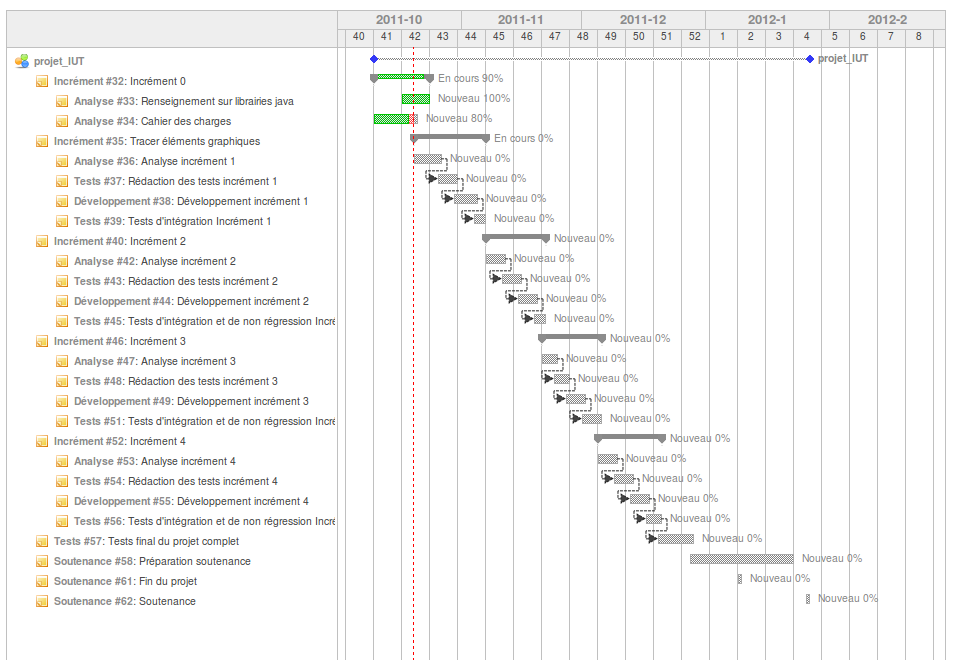
\includegraphics[height=430px, angle=-90]{projetiut-gantt.png}

\section{Glossaire}
	\paragraph{Complexité cyclomatique} Outil de métrologie logicielle permettant de mesurer la complexité d'un programme. Cette mesure comptabilise le nombre de chemin possible au travers d'un programme représenté sous la forme d'un graphe.
	\paragraph{Diagramme de classes} Schéma utilisé en génie logiciel pour représenter les classes et les interfaces des systèmes
	ainsi que les différentes relations entre celles-ci. Ce diagramme est inclus dans la partie statique d'UML.
	\paragraph{Diagramme de séquence} Représentation graphique des interactions entre les acteurs et le système selon un ordre 
	chronologique. Ce diagramme est inclus dans la partie dynamique d'UML.
	\paragraph{EDI} Environnement de Développement Intégré (ou IDE en anglais). Programme regroupant un ensemble d'outils pour développement de logiciels, un EDI
	est prévu pour simplifier la tâche du développeur et fournir des fonctionnalités supplémentaire vis-à-vis d'un éditeur de texte classique.
	\paragraph{Incrément} Fonctionnalité du logiciel, ayant un cycle logiciel lui étant propre (Analyse, Développement, Tests). Cette 
	fonctionnalité doit être opérationnelle pour que l'incrément soit terminé. Il doit améliorer le logiciel par rapport à l'incrément précédent, 
	et ne doit pas altérer les fonctionnalités précédentes.
	\paragraph{Java} Langage de programmation orienté objet moderne, il compile le programme pour ensuite l'exécuter sur une machine Java, ainsi le programme une fois
	compilé peut être exécuté sur différentes plateforme (Windows, Linux, Mac OSX, \ldots).
	\paragraph{UML} (Unified Modeling Language) Langage de modélisation graphique à base de pictogramme. Il est apparu dans un monde du génie logiciel dans le cadre de la conception orientée objet. Ce langage est composés de différents diagrammes, allant du développement à la simple analyse des besoins. 
\section{Bibliographie}
\begin{thebibliography}{1}
	\bibitem{coursUML} Thierry \bsc{Millan} Cours sur la modélisation UML, 2011 
	\bibitem{coursQualite} Thierry \bsc{Millan} Cours sur la qualitée logicielle, 2011 
	\bibitem{wikiUML} Article sur UML \url{http://fr.wikipedia.org/wiki/Unified_Modeling_Language}, 2011 
\end{thebibliography}
\end{document}
